\documentclass[]{article}
\usepackage{lmodern}
\usepackage{amssymb,amsmath}
\usepackage{ifxetex,ifluatex}
\usepackage{fixltx2e} % provides \textsubscript
\ifnum 0\ifxetex 1\fi\ifluatex 1\fi=0 % if pdftex
  \usepackage[T1]{fontenc}
  \usepackage[utf8]{inputenc}
\else % if luatex or xelatex
  \ifxetex
    \usepackage{mathspec}
  \else
    \usepackage{fontspec}
  \fi
  \defaultfontfeatures{Ligatures=TeX,Scale=MatchLowercase}
\fi
% use upquote if available, for straight quotes in verbatim environments
\IfFileExists{upquote.sty}{\usepackage{upquote}}{}
% use microtype if available
\IfFileExists{microtype.sty}{%
\usepackage{microtype}
\UseMicrotypeSet[protrusion]{basicmath} % disable protrusion for tt fonts
}{}
\usepackage[margin=1in]{geometry}
\usepackage{hyperref}
\hypersetup{unicode=true,
            pdftitle={ICL maximisation for discrete latent variable models},
            pdfauthor={Etienne Côme},
            pdfborder={0 0 0},
            breaklinks=true}
\urlstyle{same}  % don't use monospace font for urls
\usepackage{color}
\usepackage{fancyvrb}
\newcommand{\VerbBar}{|}
\newcommand{\VERB}{\Verb[commandchars=\\\{\}]}
\DefineVerbatimEnvironment{Highlighting}{Verbatim}{commandchars=\\\{\}}
% Add ',fontsize=\small' for more characters per line
\usepackage{framed}
\definecolor{shadecolor}{RGB}{248,248,248}
\newenvironment{Shaded}{\begin{snugshade}}{\end{snugshade}}
\newcommand{\KeywordTok}[1]{\textcolor[rgb]{0.13,0.29,0.53}{\textbf{#1}}}
\newcommand{\DataTypeTok}[1]{\textcolor[rgb]{0.13,0.29,0.53}{#1}}
\newcommand{\DecValTok}[1]{\textcolor[rgb]{0.00,0.00,0.81}{#1}}
\newcommand{\BaseNTok}[1]{\textcolor[rgb]{0.00,0.00,0.81}{#1}}
\newcommand{\FloatTok}[1]{\textcolor[rgb]{0.00,0.00,0.81}{#1}}
\newcommand{\ConstantTok}[1]{\textcolor[rgb]{0.00,0.00,0.00}{#1}}
\newcommand{\CharTok}[1]{\textcolor[rgb]{0.31,0.60,0.02}{#1}}
\newcommand{\SpecialCharTok}[1]{\textcolor[rgb]{0.00,0.00,0.00}{#1}}
\newcommand{\StringTok}[1]{\textcolor[rgb]{0.31,0.60,0.02}{#1}}
\newcommand{\VerbatimStringTok}[1]{\textcolor[rgb]{0.31,0.60,0.02}{#1}}
\newcommand{\SpecialStringTok}[1]{\textcolor[rgb]{0.31,0.60,0.02}{#1}}
\newcommand{\ImportTok}[1]{#1}
\newcommand{\CommentTok}[1]{\textcolor[rgb]{0.56,0.35,0.01}{\textit{#1}}}
\newcommand{\DocumentationTok}[1]{\textcolor[rgb]{0.56,0.35,0.01}{\textbf{\textit{#1}}}}
\newcommand{\AnnotationTok}[1]{\textcolor[rgb]{0.56,0.35,0.01}{\textbf{\textit{#1}}}}
\newcommand{\CommentVarTok}[1]{\textcolor[rgb]{0.56,0.35,0.01}{\textbf{\textit{#1}}}}
\newcommand{\OtherTok}[1]{\textcolor[rgb]{0.56,0.35,0.01}{#1}}
\newcommand{\FunctionTok}[1]{\textcolor[rgb]{0.00,0.00,0.00}{#1}}
\newcommand{\VariableTok}[1]{\textcolor[rgb]{0.00,0.00,0.00}{#1}}
\newcommand{\ControlFlowTok}[1]{\textcolor[rgb]{0.13,0.29,0.53}{\textbf{#1}}}
\newcommand{\OperatorTok}[1]{\textcolor[rgb]{0.81,0.36,0.00}{\textbf{#1}}}
\newcommand{\BuiltInTok}[1]{#1}
\newcommand{\ExtensionTok}[1]{#1}
\newcommand{\PreprocessorTok}[1]{\textcolor[rgb]{0.56,0.35,0.01}{\textit{#1}}}
\newcommand{\AttributeTok}[1]{\textcolor[rgb]{0.77,0.63,0.00}{#1}}
\newcommand{\RegionMarkerTok}[1]{#1}
\newcommand{\InformationTok}[1]{\textcolor[rgb]{0.56,0.35,0.01}{\textbf{\textit{#1}}}}
\newcommand{\WarningTok}[1]{\textcolor[rgb]{0.56,0.35,0.01}{\textbf{\textit{#1}}}}
\newcommand{\AlertTok}[1]{\textcolor[rgb]{0.94,0.16,0.16}{#1}}
\newcommand{\ErrorTok}[1]{\textcolor[rgb]{0.64,0.00,0.00}{\textbf{#1}}}
\newcommand{\NormalTok}[1]{#1}
\usepackage{graphicx,grffile}
\makeatletter
\def\maxwidth{\ifdim\Gin@nat@width>\linewidth\linewidth\else\Gin@nat@width\fi}
\def\maxheight{\ifdim\Gin@nat@height>\textheight\textheight\else\Gin@nat@height\fi}
\makeatother
% Scale images if necessary, so that they will not overflow the page
% margins by default, and it is still possible to overwrite the defaults
% using explicit options in \includegraphics[width, height, ...]{}
\setkeys{Gin}{width=\maxwidth,height=\maxheight,keepaspectratio}
\IfFileExists{parskip.sty}{%
\usepackage{parskip}
}{% else
\setlength{\parindent}{0pt}
\setlength{\parskip}{6pt plus 2pt minus 1pt}
}
\setlength{\emergencystretch}{3em}  % prevent overfull lines
\providecommand{\tightlist}{%
  \setlength{\itemsep}{0pt}\setlength{\parskip}{0pt}}
\setcounter{secnumdepth}{0}
% Redefines (sub)paragraphs to behave more like sections
\ifx\paragraph\undefined\else
\let\oldparagraph\paragraph
\renewcommand{\paragraph}[1]{\oldparagraph{#1}\mbox{}}
\fi
\ifx\subparagraph\undefined\else
\let\oldsubparagraph\subparagraph
\renewcommand{\subparagraph}[1]{\oldsubparagraph{#1}\mbox{}}
\fi

%%% Use protect on footnotes to avoid problems with footnotes in titles
\let\rmarkdownfootnote\footnote%
\def\footnote{\protect\rmarkdownfootnote}

%%% Change title format to be more compact
\usepackage{titling}

% Create subtitle command for use in maketitle
\providecommand{\subtitle}[1]{
  \posttitle{
    \begin{center}\large#1\end{center}
    }
}

\setlength{\droptitle}{-2em}

  \title{ICL maximisation for discrete latent variable models}
    \pretitle{\vspace{\droptitle}\centering\huge}
  \posttitle{\par}
    \author{Etienne Côme}
    \preauthor{\centering\large\emph}
  \postauthor{\par}
      \predate{\centering\large\emph}
  \postdate{\par}
    \date{23 mai 2019}


\begin{document}
\maketitle

\subsection{Abstract}\label{abstract}

\subsection{Introduction}\label{introduction}

Model based clustering is a principled approach for clustering (Fraley
and Raftery 2002), that has already proved to be very useful in a
variety of context thanks to it's capability of dealing with particular
data structures. Such approaches encompasses to name a few: Gaussian
Mixture Models (GMM), mixture of regression and graph clustering models
like Stochastic Block Models (SBM). In their basic form such models
assume that the observations \(\{x_1,...x_N\}\) are drawn from a two
step process, first a discrete latent variable is drawn using a
multinomial distribution (with proportions \(\pi\)), then conditionally
on the drawn cluster an observation is sampled using the cluster own
distribution. More formally, this can be written as:

\[
\begin{eqnarray}
\mathbf{z}_i|\pi&\sim& \mathcal{M}(1,\pi)\\
x_i|\mathbf{z}_{ik}=1,\theta_{k}&\sim& \mathcal{F}(\theta_{k}),
\end{eqnarray}
\]

where the \(\mathbf{z}_i\in\{0,1\}^K\) is the so-called latent variable
encoding cluster membership. From a computational perspective there are
two main way to deal with such type of models. From a frequentist
perspective, if the main focus is in estimating the data distribution
it's natural to integrate out the latent variable and look for the
\(\theta\) that maximize the likelihood:

\[
\begin{eqnarray}
L(\theta_1,...,\theta_K)=\prod_{i=1}^N\sum_{k=1}^{K}\pi_k f(x_i;\theta_k),
\end{eqnarray}
\] where \(f\) is the density of the mixtures component distributions.
Such functional forms are not easy to optimize but the well known EM
algorithm (Dempster, Laird, and Rubin 1977) is a natural solution to
this problem when the latent variable are independents given the
observations. When this is not the case one may resorts to variational
approximations (Jordan et al. 1999) to solve the optimization problem.
These type of approaches converge to a local maximum of the likelihood
and require the number of cluster to be fixed. When the number of groups
\(K\) is unknown, one classically try several values and resorts to
model selection criteria like BIC and AIC (McLachlan and Peel 2000) to
find the best fitting model given the data at hands. These solution
leads typically to algorithms with complexity \(\mathcal{O}(NK^2d)\)
where \(d\) is the number of features (for model selection and model
fitting).

Always from a frequentist perspective when the main goal is to recovers
the latent variable states one may keep them in the optimization problem
and try to maximize the complete data likelihood with respect to both
the latent variables states and the distributions parameters. This leads
to the Classification EM algorithm (Celeux and Govaert 1992) which
generalize the K-means algorithm (which corresponds to the special case
of a mixture of spherical Gaussian with equal proportions). Such
solution leads to algorithm with the same complexity as a classical EM
even if they may converge more quickly. Such approaches also leave open
the question of model selection (with respect to the number of mixture
component).

From a Bayesian perspective a natural way to deals with finite mixture
model come from MCMC sampling which can be used to sample both latent
variables values and parameters according to the posterior distribution.
In such setting, the mixture model is complemented with prior
distributions over parameters \((\pi,\theta_1,...,\theta_k)\), which are
often chose to be conjugate. A Dirichlet distribution being used as
prior for the latent variables. This leads to the following type of
models:

\[
\begin{eqnarray}
\pi&\sim& \mathcal{D}(\mathbf{\alpha})\\
\mathbf{z}_i|\pi&\sim& \mathcal{M}(1,\pi)\\
\theta_{k}&\sim& P(\mathbf{\beta})\\
x_i|\mathbf{z}_{ik}=1,\theta_k&\sim& \mathcal{F}(\theta_{k})
\end{eqnarray}
\]

with \(\mathcal{D}(\alpha)\) the Dirichlet distribution of parameter
\(\alpha\) and \(P(\beta)\) a prior distribution for the \(\theta\)'s.
Using Gibbs sampling (Diebolt and P. 1994) or variant one may obtain
sample from the posterior distribution. However, sampling can be hard
with difficulty to explore the different modes of the posterior
distribution. Exploration of the posterior samples can also be hard to
perform due to the label switching problem (Diebolt and P. 1994,Stephens
(2000)) and even difficulties in retrieving the more plausible latent
variable state (Rastelli and Friel 2018). For a more complete discussion
of these different approaches and a complete state of the art on these
problem see (Celeux, Fruewirth-Schnatter, and Robert 2018).

In between the frequentist and the Bayesian approaches several works
introduced at the begining for model selection purposes the Integrated
claffification likelihood (ICL), which correspond to the marginalisation
of the model over it's parameters leaving solely the data, the latent
variables and the priors parameters:

\[
\begin{eqnarray}
ICL(X,Z;\alpha,\beta) = \log(p(X,Z|\alpha,\beta)) &=& \log\left(\int_{\theta}\int_{\pi}p(x|z,\theta)p(\theta|\beta)p(z|\pi)p(\pi|\alpha)d\theta d\pi\right)\\
&=&\log\left(\int_{\pi}p(z|\pi)p(\pi|\alpha)d\pi\right)+\log\left(\int_{\theta}p(x|z,\theta)p(\theta|\beta)d\theta\right)
\end{eqnarray}
\] Approximate ICL criterion were first introduce and correspond to a
BIC like approximation of this integral with improper and non
informative prior. Note that ICL was originally proposed by Biernacki,
Celeux and Govaert (Biernacki, Celeux, and Govaert 2000) for Gaussian
mixture models. It was then adapted by Biernacki, Celeux and Govaert
(Biernacki, Celeux, and Govaert 2010) to mixtures of multivariate
multinomial distributions and to the SBM model by Daudin, Picard and
Robin (Daudin, Picard, and Robin 2008).

Eventually, a new line of work was started by working directly with an
exact version of the ICL criterion derived in a complete Bayesian
setting with conjugate priors, which can in some cases be defined as
uninformative. First the exact criterion was derived for mixture of
multinomial in (Biernacki, Celeux, and Govaert 2010) but still used only
for model selection purposes in conjunction with a classical EM
algorithm. Then, greedy heuristics were successfully tested to directly
optimize this criterion over the space of possible partitions avoiding
the use of EM like algorithm as a first step. Such type of algorithm
performs model selection and clustering at the same time and are
computationaly attractive with a . This approach was introduced in (Côme
and Latouche 2015) for SBM models and then used in other type of context
(Bertoletti, Friel, and Rastelli 2015,Corneli, Latouche, and Rossi
(2016),Zreik, Latouche, and Bouveyron (2017)). This paper elaborate on
this line of work and propose two main contributions:

\begin{itemize}
\item
  An hybrid algorithm which use evolutionary strategy and local search
  for optimizing the ICL criterion is introduced. This algorithm is
  adaptable to a variety of mixture model as soon as swap and merge move
  can be efficiently computed. This algorithm is tested in real and
  simulated test cases and for a variety of mixture model namely:
  mixture of Gaussian, SBM, degree-corrected SBM.
\item
  We propose a general heuristic for extracting a regularization path
  with respect to \(\alpha\). This strategy enable the extraction of a
  dendogramme and a partial ordering of the cluster which is interesting
  on real data-sets and for visualisation purposes. Since it allow to
  study different solution of diminishing complexity and supply a
  partial ordering usefull to .
\end{itemize}

As a motivating example for the proposed solution we simulate a random
SBM graph with 1500 nodes and a hierarchical cluster structure with 3
big clusters composed of 5 swmall cluster and present the result of a
greedy opitmisation with a random starting partition with twenty
clusters. The results of the proposed hybrid optimization algorithm and
the results after reordoning obtained with the regularisation path
exatraction heuristic.

\begin{Shaded}
\begin{Highlighting}[]
\NormalTok{N=}\DecValTok{1500}
\NormalTok{K=}\DecValTok{15}
\NormalTok{pi=}\KeywordTok{rep}\NormalTok{(}\DecValTok{1}\OperatorTok{/}\NormalTok{K,K)}
\NormalTok{lambda  =}\StringTok{ }\FloatTok{0.1}
\NormalTok{lambda_o =}\StringTok{ }\FloatTok{0.025}
\NormalTok{Ks=}\DecValTok{5}
\NormalTok{mu =}\StringTok{ }\KeywordTok{bdiag}\NormalTok{(}\KeywordTok{lapply}\NormalTok{(}\DecValTok{1}\OperatorTok{:}\NormalTok{(K}\OperatorTok{/}\NormalTok{Ks), }\ControlFlowTok{function}\NormalTok{(k)\{}\KeywordTok{matrix}\NormalTok{(lambda_o,Ks,Ks)}\OperatorTok{+}\KeywordTok{diag}\NormalTok{(}\KeywordTok{rep}\NormalTok{(lambda,Ks))\}))}\OperatorTok{+}\FloatTok{0.001}
\NormalTok{sbm =}\StringTok{ }\KeywordTok{rsbm}\NormalTok{(N,pi,mu)}
\end{Highlighting}
\end{Shaded}

\begin{figure}
\centering
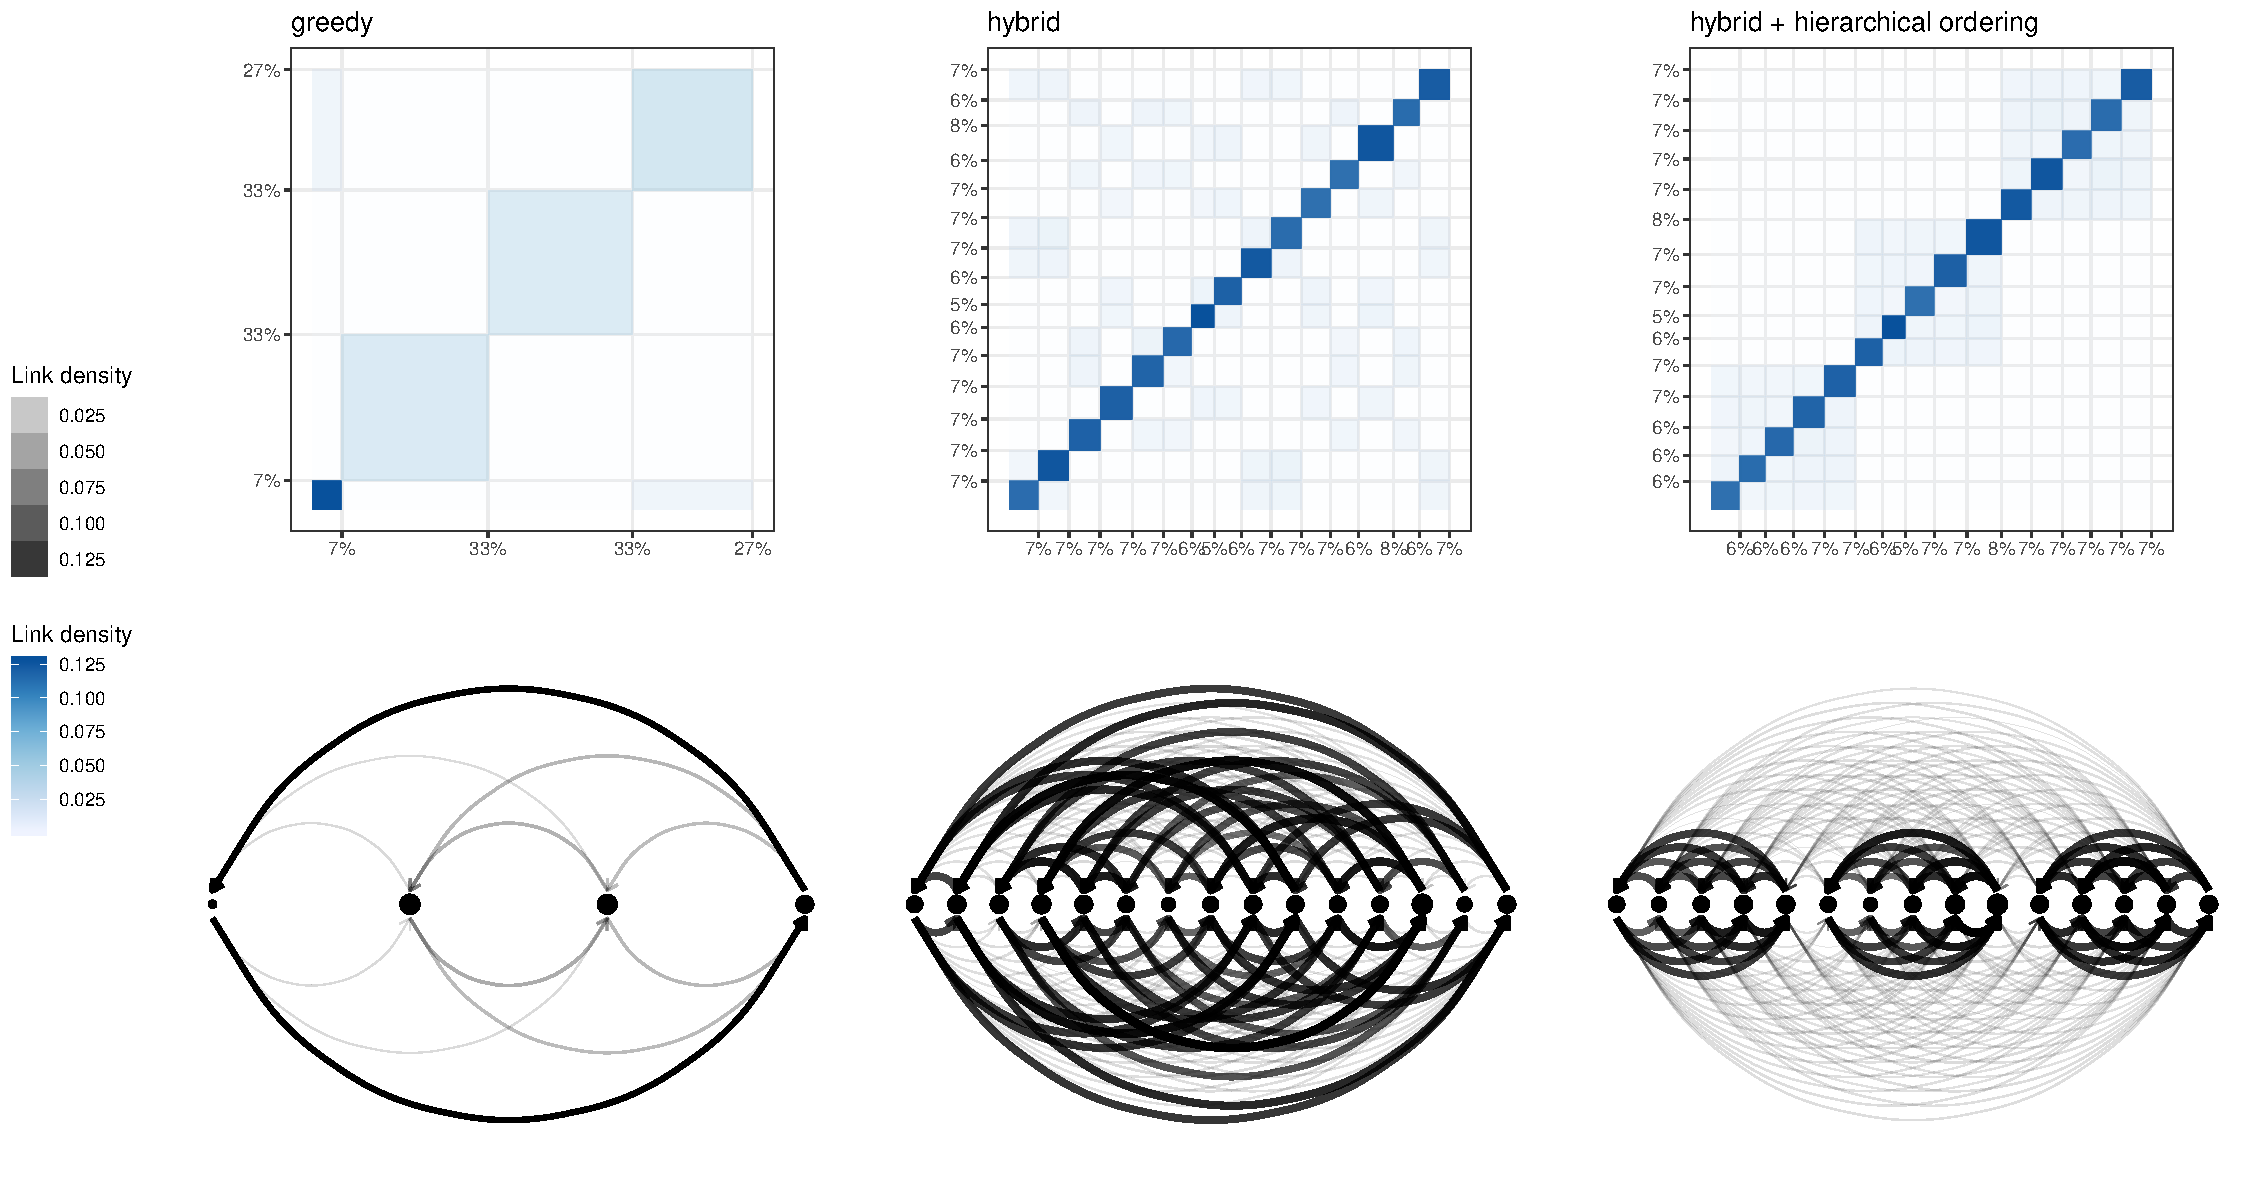
\includegraphics{paper_files/figure-latex/unnamed-chunk-4-1.pdf}
\caption{Motivating example of the proposed algorithm. Block matrix
representation of the solutions upper row and cluster node link diagram}
\end{figure}

As clearly shown by this example greedy heuristic with random strating
point suffers from under-fitting with only 4 clusters extracted among
the 15 simulated. The hybrid algorithm did not suffer from under-fitting
in this example and the hierachical ordering enable clear visualisation
of the hierachical structure of this dataset.

This paper is organized as follow, first the ICL criterions for some
mixture model are detailled, in particular in the graph clustering
context where the partition apply to both the rows and colums of the
data-matrix. Then, the proposed optimization strategy is described and
tested in sereval simulated and real test cases and compared with
possible alternatives. Eventualy, the heuristic to extract a
redularization path over \(\alpha\) is introduced and it's interest in
real situation demonstrated. Prior to some words on related works and
concluding remarks.

\subsubsection{Models and criterions}\label{models-and-criterions}

\paragraph{Mixture of multinomial}\label{mixture-of-multinomial}

\paragraph{Mixture of regression with gaussian mixture as special
case}\label{mixture-of-regression-with-gaussian-mixture-as-special-case}

\paragraph{Stochastick block models and it's degree corected
version}\label{stochastick-block-models-and-its-degree-corected-version}

\subsubsection{Optimization Algorithms}\label{optimization-algorithms}

Current solution to optimize directly ICL type criterions are mainly
based on greedy hill climbing algorithms (Côme and Latouche
2015,Bertoletti, Friel, and Rastelli (2015),Corneli, Latouche, and Rossi
(2016),Wyse, Friel, and Latouche (2017),Zreik, Latouche, and Bouveyron
(2017)). Starting from a carrefully chosen over-segmented initial
partition (build using k-means for example), swap and eventually merge
moved are appplied to increase the criterion. During the process cluster
can die enabling model selection with respect to the number of cluster.
These algorithms are quite easy to set up, computationaly attractive and
give quite good results. The major drawback of this approach is it's
dependancy to the quality of the starting partition. When random
initialization is used and the clustering structure is not easy to
extract such algorithms may lead to under-fitting as demonsatred in the
introductory example. To deal with this limitation, one potential path
to investigate come from meta-heuristics which thanks to their more
global nature could be a way to solve this problem. Following this idea
we tried to mix the greedy local search heuristic already proposed with
genetic algorithms.

Genetic algorithms evolve a population of solutions by selecting some of
the more promising ones, crossing them, possibly mutating them until a
specified number of generation or other stopping criterion is met. The
main component of these algorithms are the solution representation, the
selection strategie and the operators used for cross-over and mutation.
To represent a solution which in our case is a partition one classicaly
use a vector of cluster index. This representation will be valid for all
the models, whereas other based for example on list of prototypes would
only works for some models. The fact that this representation will works
with all of the model leads us to stick with it. However since our
optimization problem is over partitions and that our cost function is
invariant under permutation of the class label (label switching) this
representation is redundant and this fact have an important impact on
the design of the recombination (crossover) operator. Simple
recombination operators based on crossover points will not take this
particularity into account and completly break the structure of the
solution, leading to slow evolution of the population of solutions. To
circumvent this problem we looked at another solution for crossing to
partitions that will not breaks the found structures. The main idea of
our proposal is based around the the cross partition. The cross
partition of two partition is simply the partition build by considering
all the possible intersections between the elements of the two
partitions being crossed. More formally: \[
\mathcal{P}^1\times\mathcal{P}^2 := \{S^1_i \cap S^2_j \,,\, \forall i\in \{1,...,|\mathcal{P}^1|\}, j\in \{1,...,|\mathcal{P}^2|\}\}\setminus \emptyset,
\] with \(\mathcal{P}^1=\{S_1^1,...,S^1_{K_1}\}\) and
\(\mathcal{P}^2=\{S_1^2,...,S^2_{K_2}\}\) two partitions of
\([1,...,N]\). Using this operator on two solutions will produce a new
solution wich is refinement of both crossed partitions and with at most
\(|\mathcal{P}^1|\times|\mathcal{P}^1|\) clusters. In practice, the two
solutions being merge will aggree on some clusters and the number of new
clusters after crossing will be smaller than this value. As an example
if we take two solutions obtained with local greedy search on the
introductory example, they suffers from underfiting with 7 and 6
clusters each among the 15 of the simulations and a normalized mutual
information (NMI) with the simulated labels of 0.56 and 0.56
respectively. If now, we cross these two solutions we get a new solution
with 10 clusters (much smaller than the 42 potential that we would have
obtained if the two partitions were completly differents) and an NMI of
0.76. Therefore, in case of under-fitting of both parents partition
crossing alone will already improve the solution. This operators may
create superflous clusters when the solution are around the best one,
but greedy local search can be used to remove these superfluous clusters
and this operator seems therefore a good proposal for combination with
greedy local search in particular with merge move. The remaining
question concerns the selection procedures used and the mutation
operators. For the selection process we tested several solutions which
did not changed too much the performances of the algorithm and
eventually used rank selection {[}{]}, for the mutation operator

\begin{verbatim}
Build a population of initial solution using greedy swap
while nb_generation < nb_max_generation 
  sample according to their rank (pop_size - 1) pairs of solution in the population 
  add the best solution in the population to the new generation
  for each pairs of partitions
    build the cross partition
    try to update the new partition using greedy merge
    if random number < probability of mutation
      sample a cluster and split it randomly in two new clusters
    try to update the new partition using greedy swap
    add the partition to the new generation
  set the population to the build new generation
return the best solution found
\end{verbatim}

\paragraph{Computational efficiency and constrained
moves}\label{computational-efficiency-and-constrained-moves}

\paragraph{Experiments}\label{experiments}

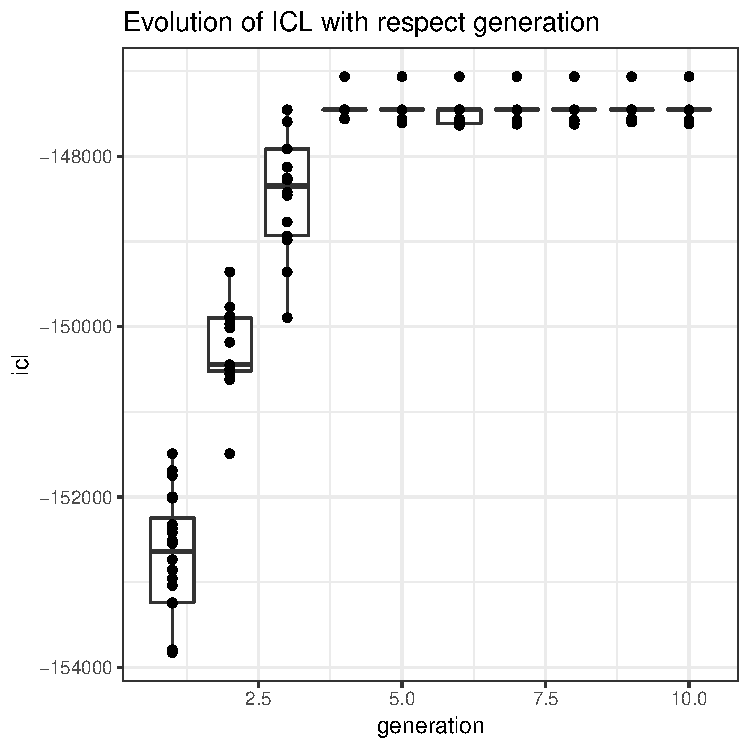
\includegraphics{paper_files/figure-latex/unnamed-chunk-5-1.pdf}

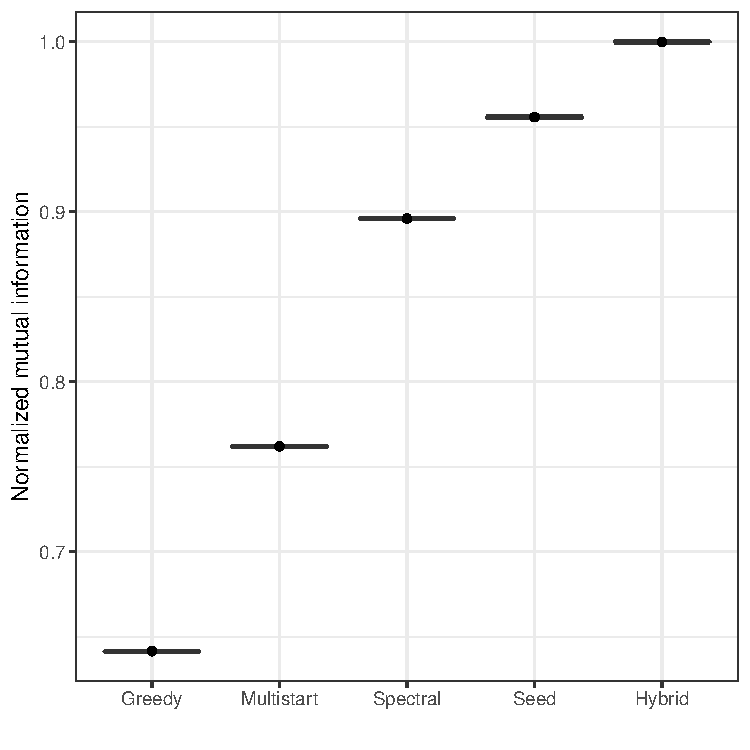
\includegraphics{paper_files/figure-latex/unnamed-chunk-7-1.pdf}

\subsection{Regularisation path and hierarchical
clustering}\label{regularisation-path-and-hierarchical-clustering}

\subsubsection{Real data}\label{real-data}

\begin{Shaded}
\begin{Highlighting}[]
\KeywordTok{data}\NormalTok{(}\StringTok{"Blogs"}\NormalTok{)}
\NormalTok{fit_blogs =}\StringTok{ }\KeywordTok{greed}\NormalTok{(Blogs}\OperatorTok{$}\NormalTok{X,}\DataTypeTok{model=}\KeywordTok{new}\NormalTok{(}\StringTok{"dcsbm"}\NormalTok{))}
\KeywordTok{data}\NormalTok{(}\StringTok{"Books"}\NormalTok{)}
\NormalTok{fit_books =}\StringTok{ }\KeywordTok{greed}\NormalTok{(Books}\OperatorTok{$}\NormalTok{X,}\DataTypeTok{model=}\KeywordTok{new}\NormalTok{(}\StringTok{"dcsbm"}\NormalTok{))}
\KeywordTok{data}\NormalTok{(}\StringTok{"Football"}\NormalTok{)}
\NormalTok{fit_foot =}\StringTok{ }\KeywordTok{greed}\NormalTok{(Football}\OperatorTok{$}\NormalTok{X,}\DataTypeTok{model=}\KeywordTok{new}\NormalTok{(}\StringTok{"dcsbm"}\NormalTok{))}
\KeywordTok{data}\NormalTok{(}\StringTok{"Jazz"}\NormalTok{)}
\NormalTok{fit_jazz =}\StringTok{ }\KeywordTok{greed}\NormalTok{(Jazz,}\DataTypeTok{model=}\KeywordTok{new}\NormalTok{(}\StringTok{"dcsbm"}\NormalTok{))}
\end{Highlighting}
\end{Shaded}

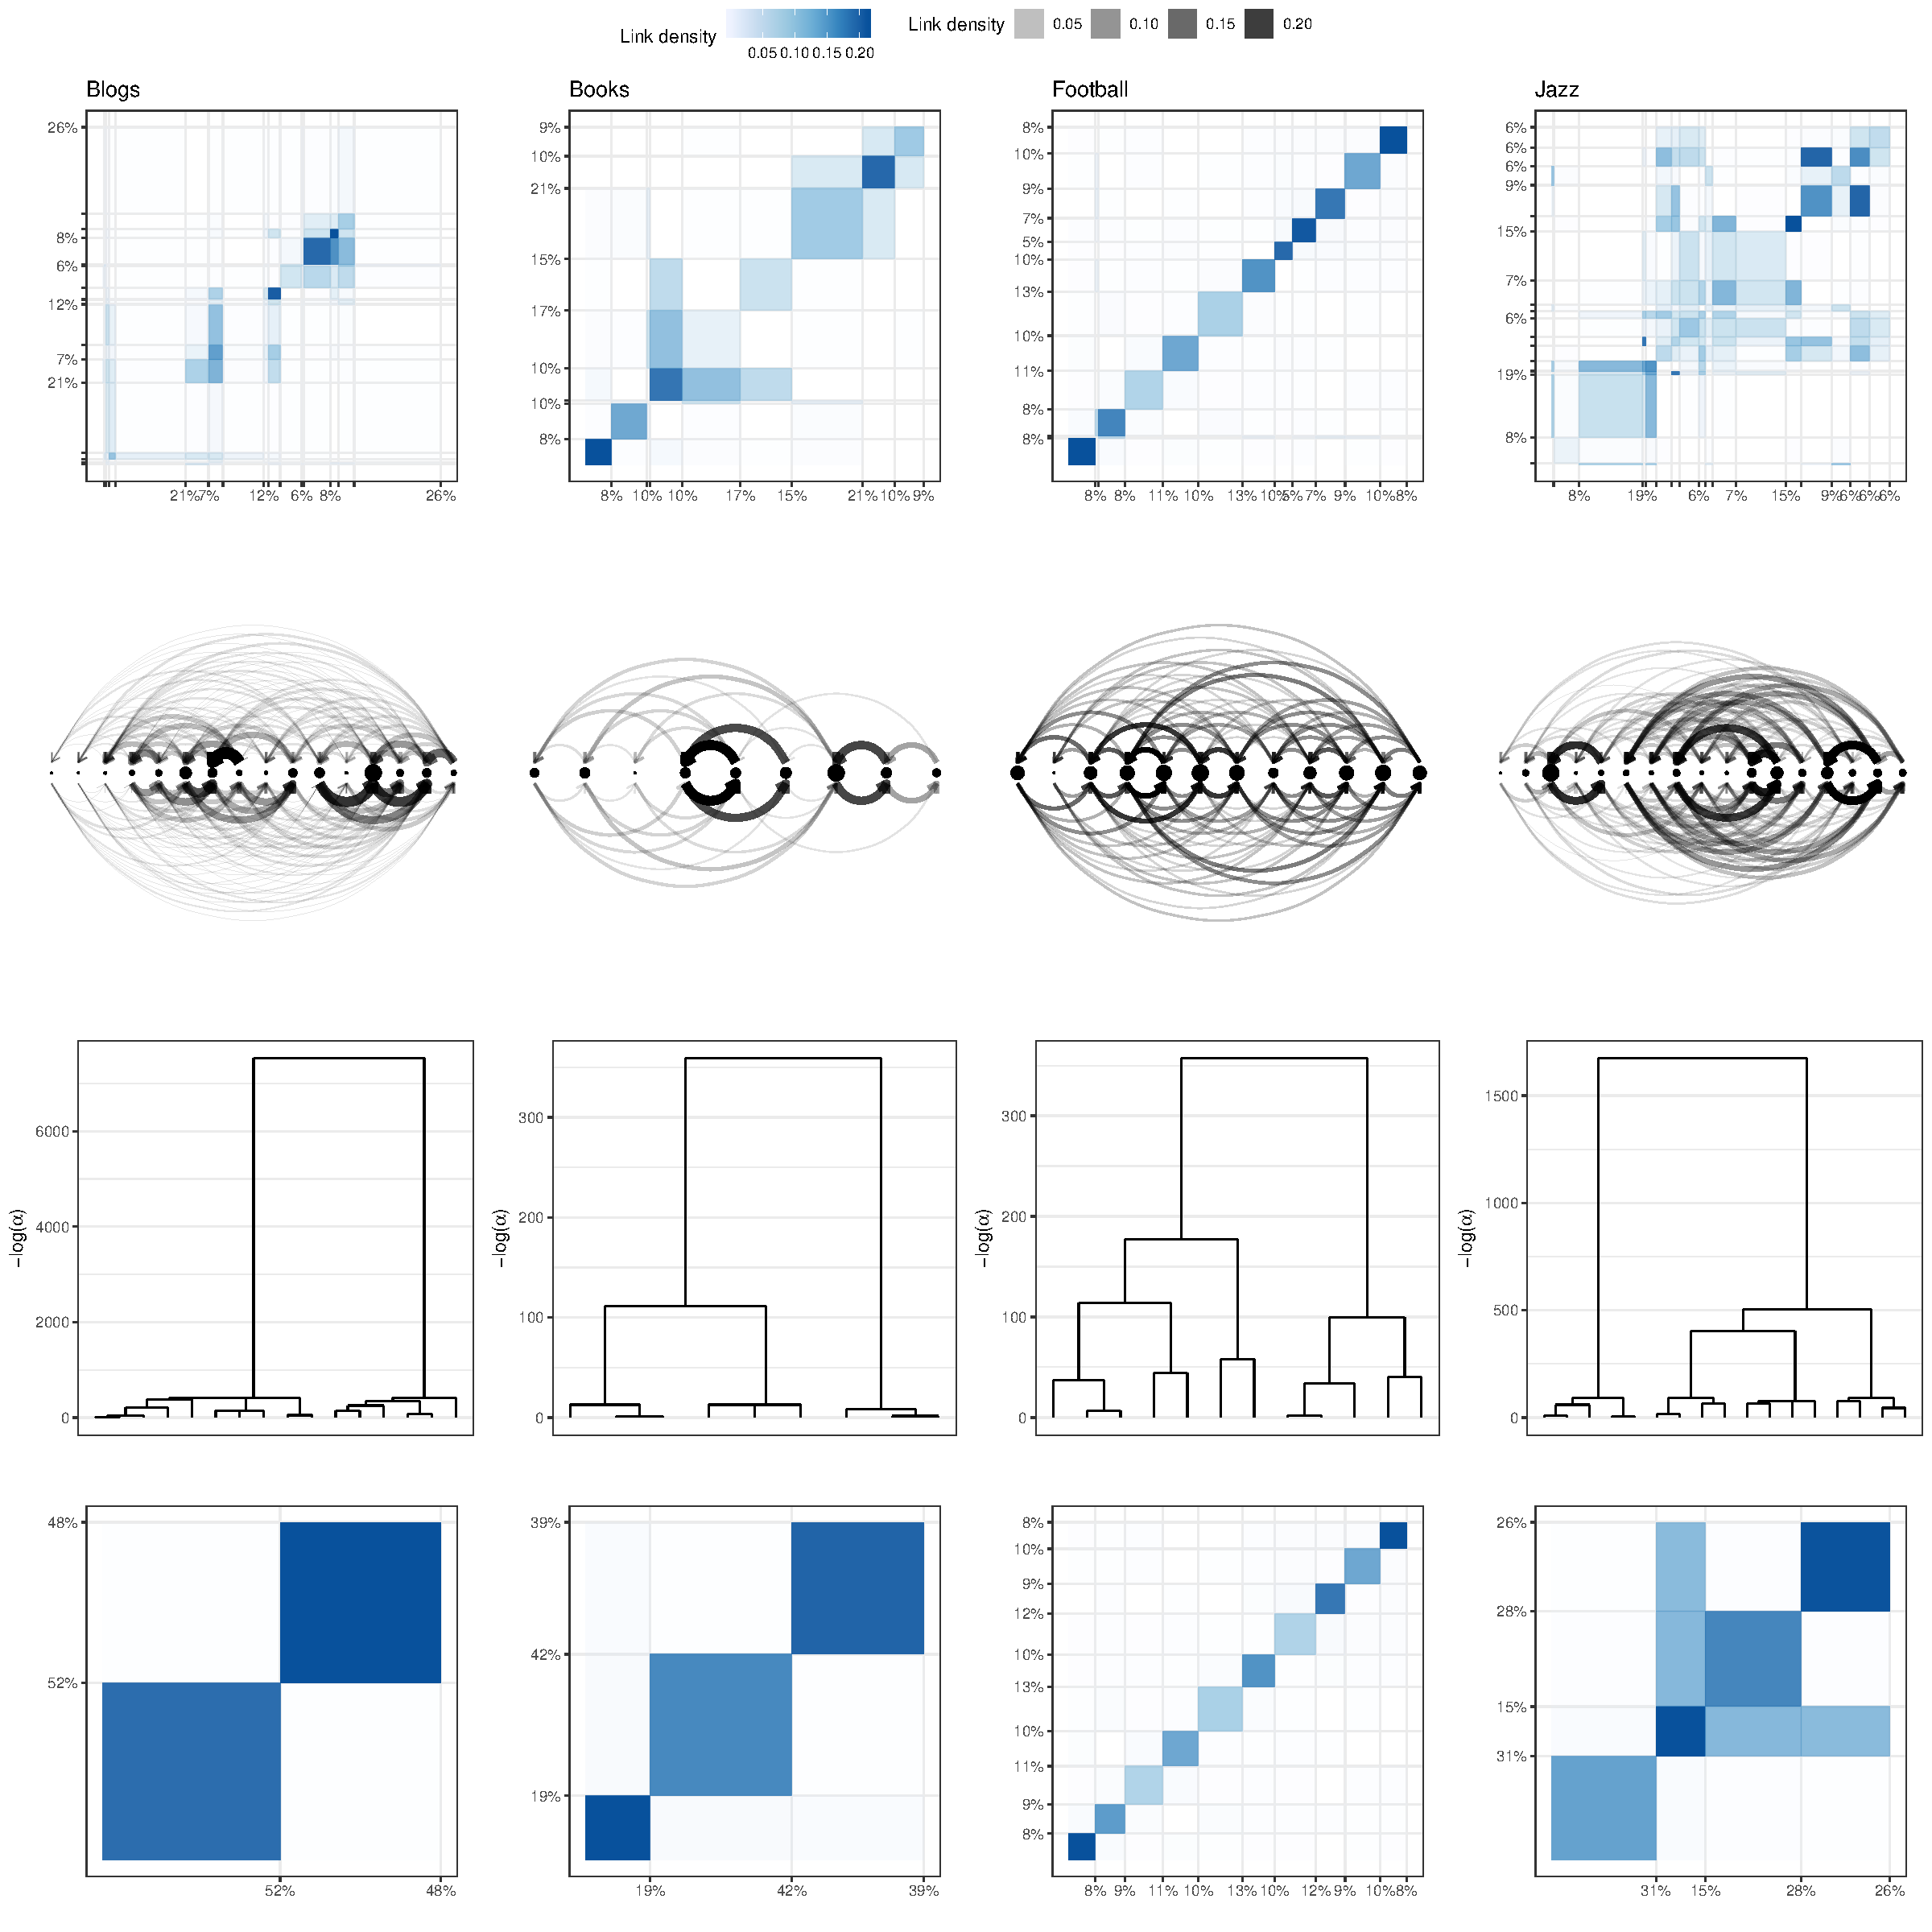
\includegraphics{paper_files/figure-latex/unnamed-chunk-8-1.pdf} \#\#
Related works and conclusions

\subsection{Conclusion}\label{conclusion}

\subsection*{References}\label{references}
\addcontentsline{toc}{subsection}{References}

\hypertarget{refs}{}
\hypertarget{ref-Bertoletti2015}{}
Bertoletti, Marco, Nial Friel, and Riccardo Rastelli. 2015. ``Choosing
the Number of Clusters in a Finite Mixture Model Using an Exact
Integrated Completed Likelihood Criterion.'' \emph{METRON} 73 (2):
177--99.
doi:\href{https://doi.org/10.1007/s40300-015-0064-5}{10.1007/s40300-015-0064-5}.

\hypertarget{ref-Biernacki2000}{}
Biernacki, Christophe, Gilles Celeux, and Gerard Govaert. 2000.
``Assessing a Mixture Model for Clustering with the Integrated Completed
Likelihood.'' \emph{IEEE Transaction on Pattern Analysis and Machine
Intelligence} 7: 719--25.

\hypertarget{ref-Biernacki2010}{}
---------. 2010. ``Exact and Monte Carlo Calculations of Integrated
Likelihoods for the Latent Class Model.'' \emph{Journal of Statistical
Planning and Inference} 140: 2991--3002.

\hypertarget{ref-Celeux92}{}
Celeux, Gilles, and Gerard Govaert. 1992. ``A Classification Em
Algorithm for Clustering and Two Stochastic Versions.''
\emph{Computational Statistics \& Data Analysis} 14 (3): 315--32.
\url{https://EconPapers.repec.org/RePEc:eee:csdana:v:14:y:1992:i:3:p:315-332}.

\hypertarget{ref-Celeux2018}{}
Celeux, Gilles, Sylvia Fruewirth-Schnatter, and Christian P. Robert.
2018. ``Model Selection for Mixture Models - Perspectives and
Strategies.'' \emph{arXiv E-Prints}, December, arXiv:1812.09885.

\hypertarget{ref-Corneli2016}{}
Corneli, Marco, Pierre Latouche, and Fabrice Rossi. 2016. ``Exact Icl
Maximization in a Non-Stationary Temporal Extension of the Stochastic
Block Model for Dynamic Networks.'' \emph{Neurocomputing} 192: 81--91.
doi:\href{https://doi.org/https://doi.org/10.1016/j.neucom.2016.02.031}{https://doi.org/10.1016/j.neucom.2016.02.031}.

\hypertarget{ref-Come2015}{}
Côme, Etienne, and Pierre Latouche. 2015. ``Model Selection and
Clustering in Stochastic Block Models Based on the Exact Integrated
Complete Data Likelihood.'' \emph{Statistical Modelling} 15 (6):
564--89.
doi:\href{https://doi.org/10.1177/1471082X15577017}{10.1177/1471082X15577017}.

\hypertarget{ref-Daudin2008}{}
Daudin, J., F. Picard, and S. Robin. 2008. ``A Mixture Model for Random
Graph.'' \emph{Statistics and Computing} 18: 1--36.

\hypertarget{ref-Dempster77}{}
Dempster, A. P., N. M. Laird, and D. B. Rubin. 1977. ``Maximum
Likelihood from Incomplete Data via the Em Algorithm.'' \emph{Journal of
the Royal Statistical Society. Series B (Methodological)} 39 (1).
{[}Royal Statistical Society, Wiley{]}: 1--38.
\url{http://www.jstor.org/stable/2984875}.

\hypertarget{ref-Diebolt1994}{}
Diebolt, J., and Robert C. P. 1994. ``Estimation of Finite Mixture
Distributions Through Bayesian Sampling.'' \emph{Journal of the Royal
Statistical Society B} 56: 363--75.

\hypertarget{ref-Fraley2002}{}
Fraley, Chris, and Adrian E Raftery. 2002. ``Model-Based Clustering,
Discriminant Analysis, and Density Estimation.'' \emph{Journal of the
American Statistical Association} 97 (458). Taylor \& Francis: 611--31.
doi:\href{https://doi.org/10.1198/016214502760047131}{10.1198/016214502760047131}.

\hypertarget{ref-Jordan1999}{}
Jordan, Michael I., Zoubin Ghahramani, Tommi S. Jaakkola, and Lawrence
K. Saul. 1999. ``An Introduction to Variational Methods for Graphical
Models.'' \emph{Mach. Learn.} 37 (2). Hingham, MA, USA: Kluwer Academic
Publishers: 183--233.
doi:\href{https://doi.org/10.1023/A:1007665907178}{10.1023/A:1007665907178}.

\hypertarget{ref-McLachlan2000}{}
McLachlan, Geoffrey, and David Peel. 2000. \emph{Finite Mixture Models}.
John Wiley \& Sons, Inc.
doi:\href{https://doi.org/10.1002/0471721182}{10.1002/0471721182}.

\hypertarget{ref-Rastelli2018}{}
Rastelli, Riccardo, and Nial Friel. 2018. ``Optimal Bayesian Estimators
for Latent Variable Cluster Models.'' \emph{Statistics and Computing} 28
(6): 1169--86.
doi:\href{https://doi.org/10.1007/s11222-017-9786-y}{10.1007/s11222-017-9786-y}.

\hypertarget{ref-Stephens2000}{}
Stephens, Matthew. 2000. ``Dealing with Label Switching in Mixture
Models.'' \emph{Journal of the Royal Statistical Society B} 62 (4):
795--809.

\hypertarget{ref-Wyse2017}{}
Wyse, Jason, Nial Friel, and Pierre Latouche. 2017. ``Inferring
Structure in Bipartite Networks Using the Latent Blockmodel and Exact
Icl.'' \emph{Network Science} 5 (1). Cambridge University Press: 45--69.
doi:\href{https://doi.org/10.1017/nws.2016.25}{10.1017/nws.2016.25}.

\hypertarget{ref-Zreik2017}{}
Zreik, Rawya, Pierre Latouche, and Charles Bouveyron. 2017. ``The
Dynamic Random Subgraph Model for the Clustering of Evolving Networks.''
\emph{Computational Statistics} 32 (2): 501--33.
doi:\href{https://doi.org/10.1007/s00180-016-0655-5}{10.1007/s00180-016-0655-5}.


\end{document}
